\documentclass{report}
\usepackage{graphicx}
\usepackage{float}
\usepackage{tabularx, ragged2e}
\newcommand{\n}[1]{\overline{#1}}
\newcommand{\subsubsubsection}[1]{\paragraph{#1}\mbox{}\\}
\setcounter{secnumdepth}{4}
\setcounter{tocdepth}{4}
\title{%
    Progettazione di sistemi digitali \\    
    \large Corso del professore Pontarelli
}
\author{Lugini Andrea}
\begin{document}
\maketitle
\tableofcontents
\newpage
\section{Binary numeric system}
    \subsection{Legenda}
        \begin{itemize}
            \item \textbf{a}: cifra
            \item \textbf{i}: posizione della cifra all'interno della stringa
            \item \textbf{N}: lunghezza della stringa
        \end{itemize}
    \subsection{Potenze del due}
        \begin{itemize}
            \item $2^0 = 1$
            \item $2^1 = 2$
            \item $2^2 = 4$
            \item $2^3 = 8$
            \item $2^4 = 16$
            \item $2^5 = 32$
            \item $2^6 = 64$
            \item $2^7 = 128$
            \item $2^8 = 256$
            \item $2^9 = 512$
            \item $2^{10} = 1024$
            \item $2^{11} = 2048$
            \item $2^{12} = 4096$
            \item $2^{13} = 8192$
            \item $2^{14} = 16384$
            \item $2^{15} = 32768$
            \item $2^{16} = 65536$
            \item $2^{32} = 4294967296$
            \item $2^{64} = 18446744073709551616$
        \end{itemize}
    \subsection{Il sistema binario}
        Il sistema binario è un sistema di rappresentazione dei numeri in base
        \textbf{2}, dove le uniche cifre disponibili sono \textbf{0} e \textbf{1} 
        e sono identificati da un \textbf{pedice 2}. \\
        Questo metodo è quello usato nei calcolatori digitali in quanto facilmente
        rappresentabile a livello elettronico (ON = 1, OFF = 0) tramite l'uso dei bit. \\
        $R = [0, \: 2^N - 1] \\
        \#R = 2^N$
    \subsection{Il sistema esadecimale}
        Sistema di rappresentazione in base 16, le cifre disponibili vanno da
        \textbf{0} a \textbf{F}, con le cifre da \textbf{A} fino a \textbf{F}
        che corrispondono ai valori decimali da \textbf{10} a \textbf{15}. \\
        Sono identificati da un \textbf{pedice 16}. \\
        Il valore di una cifra è dato dalla formula $valore = a_i * 2^i$. \\
        \textbf{N.B.}: Ad una cifra esadecimale corrispondono 4 cifre binarie.
    \subsection{Conversioni fra binario, decimale ed esadecimale}
        \begin{itemize}
            \item \textbf{B $\Longrightarrow$ D}: $\Sigma_{i=0}^{N-1} a_i * 2^i$.
            \item \textbf{H $\Longrightarrow$ D}: $\Sigma_{i=0}^{N-1} a_i * 16^i$.
            \item \textbf{D $\Longrightarrow$ B}: esistono 2 metodi, quello metodo della \textbf{divisione} 
                ed il metodo della \textbf{sottrazione}.
            \item \textbf{D $\Longrightarrow$ H}: Uguale a D $\Longrightarrow$ B, ma usando 16 anzichè 2.
            \item \textbf{B $\Longrightarrow$ H}: Fare gruppi di 4 cifre (da ora in poi dette bit) alla volta, 
                applicare il metodo B $\Longrightarrow$ D e convertire il valore decimale 
                con la corrispondente cifra esadecimale
            \item \textbf{H $\Longrightarrow$ B}: Prendere il valore decimale corrispondente all singola cifra e
                convertirlo in binario col metodo B $\Longrightarrow$ D 
        \end{itemize}
    \subsection{Rappresentazione binaria di numeri con segno}
        \subsubsection{Sign/Magnitude}
            Il \textbf{primo bit} è usato per memorizzare il segno (0 = +, 1 = -). \\
            I restanti bit sono usati per memorizzare il valore assoluto del numero. \\
            $R = [-(2^{N-1}) + 1, \: 2^{N-1} - 1] \\
            \#R = 2^N - 1
            $ \\
            \textbf{N.B.}: Il numero 0 è memorizzato 2 volte, come +0 e -0. \\
            Nonostante sia semplice rappresentare i numeri in questo formato, diventa
            molto più complesso farci l'operazione binaria base, l'addizione, in quanto
            non segue lo stesso modello della classica addizione binaria. E' perciò
            raramente usato.
            $$ x = a_{N-1} * (-1) * \Sigma_{i = 0}^{N-2} a_i * 2^i $$
        \subsubsection{Two's complement}
            Metodo effettivamente utilizzato per la rappresentazione dei numeri con segno.
            Il \textbf{MSB} rappresenta il valore $-(2^N-1)$, i restanti bit rappresentano 
            la "parte positiva" del numero. \\
            $R = [-(2^{N-1}), \: 2^{N-1} - 1] \\
            \#R = 2^N
            $ \\
            $$ x = a_{N-1} * -(2^N-1) + \Sigma_{i = 0}^{N-2} a_i * 2^i $$
            Con questo metoodo l'addizione si svolge come i classici numeri binari, 
            prestando però attenzioni a errori di \textbf{overflow}.
            Se sommando due numeri \textbf{concordi} otteniamo un numero a loro \textbf{discordo}
            vuol dire che abbiamo avuto un errore di \textbf{out of range}, in quanto la somma
            di questi valori ci ha portato fuori dal range rappresentabile con i bit a nostra
            disposizione.
            L'operazione \textbf{taking the two's complement} è l'operazione di
            \textbf{inversione di segno} di un valore in two's complement.
            \begin{itemize}
                \item \textbf{Invertire} i bit
                \item \textbf{Sommare 1}
            \end{itemize}
            In two's complement a volte possono capitarci degli errori di overflow, ad 
            esempio sommando un numero al suo inverso, dove possiamo però \textbf{trascurare 
            il bit di overflow}. Dobbiamo però sempre prestare attenzione al 
            \textbf{segno} del risultato per vedere se è corretto in base al segno 
            degli operandi e l'operazione eseguita. Se, per esempio, moltiplicando
            un numero positivo ed uno negativo ci ritroviamo un risultato positivo
            sappiamo di essere incorsi in un errore.
    \subsection{Rimediare all'overflow}
        Entrambi i metodi si basano sull'estensione dei bit da N ad M, con M $>$ N.
        \subsubsection{Sign-extension}
            Metodo usato per i numeri con rappresentazione \textbf{two's complement},
            consiste nell'estendere il \textbf{MSB} in tutti i nuovi bit.
        \subsubsection{Zero-extension}
            Metodo usato per gli \textbf{unsigned}, consiste nell'estendere il 
            valore \textbf{0} a tutti i nuovi bit. \\
            Leggermente diverso per i numeri in formato \textbf{Sign/Magnitude}, 
            dove il \textbf{MSB} viene lasciato con lo stesso valore pre-estensione.
    \newpage
    \subsection{Moltiplicazione}
        La moltiplicazione in binario per i numeri in \textbf{two's complement ed unsigned}
        funziona come la moltiplicazione posizionale decimale.
    \subsection{Shift}
        Caso particolare sono gli shift, dove si moltiplica per le potenze del \textbf{2}. \\
        Anche qui bisogna prestare attenzione agli overflow ed errori di segno.
        \subsubsection{Left shift}
            $$A << N = A * 2^N$$
            Basta aggiungere \textbf{N 0} in coda alla stringa binaria
        \subsubsection{Right shift}
            $$A >>> N = A * 2^{-N}$$
            Per \textbf{two's complement} e \textbf{unsigned} basta aggiungere
            \textbf{N MSB} in testa alla stringa binaria. \\
            Per i numeri \textbf{Sign/Magnitude} si aggiungono \textbf{N-1 0} e
            si lascia il \textbf{MSB} Uguale.
    \newpage
    \subsection{Frazioni e divisione}
    Il metodo di conversione da base decimale è il seguente:
    \begin{enumerate}
            \item Separare la parte intera da quella frazionaria
            \item Convertire la parte intera
            \item Moltiplicare la parte frazionaria per 2
            \item Se $p < 1 \Longrightarrow 0$. \\
                Se $p \geq 1 \Longrightarrow 1, p = p - 1$.
            \item Se $p \neq 0$ tornare al punto 4.
    \end{enumerate} 
    Diventa problematica però la rappresentazione dei numeri con la virgola. \\
    Esistono 2 metodi.
    \subsection{Fixed Point}
        Si decide a priori quanti bit per la parte intera e quanti per la parte decimale. \\
        Precisione = $2^{-N}$.
    \subsection{Floating points}     
        Notazione generica (anche detta scientifica): $\pm M * B^E$     
        Standardizzato da IEEE 754, il modello binario si basa sulla formula:
        $$1,m * 2^{e-127}$$
        Un floating point a 32 bit è memorizzato in memoria secondo il layout:
        \begin{itemize}
            \item 1 bit: segno
            \item 2-9 bit: esponente
            \item 10-32: mantissa
        \end{itemize}
        Poichè lavoriamo in sistema binario e il numero è memorizzato
        in forma \textbf{normalizzata}, sappiamo che
        l'1 prima della virgola è sempre presente e quindi \textbf{non memorizzato}. \\
        Il metodo di conversione è il seguente:
        \begin{enumerate}
            \item Convertire il numero da decimale in binario
            \item Rappresentarlo in notazine normalizzata, memorizzando di quanto
                abbiamo "spostato" la virgola
            \item Settare il primo bit in base al segno del numero
            \item Memorizzare nei bit per l'esponente lo "spostamento" $+ 127$
            \item Memorizzare nei bit della mantissa
                il numero normalizzato ignorando l'\textbf{MSB}
        \end{enumerate}
        Esistono poi dei casi speciali:
        \begin{center}
            \begin{tabular}{|c|c|c|c|}
                \hline
                Valore rappresentato & Sign bit & Exponent bits & Mantissa bits  \\
                \hline
                0 & X & All 0 & 0 \\
                \hline
                $\infty$ & 0 & All 1 & 0 \\
                \hline
                $- \infty$ & 1 & All 1 & 0 \\
                \hline
                NaN & X & All 1 & $\neq 0$ \\
                \hline
                $(-1)^s * 2^{1-bias} * 0.m$ & X & All 0 & $\neq 0$ \\
                \hline
            \end{tabular}
        \end{center}
        Esiste un motivo ben preciso per il quale nell'ultimo caso e $=-126$
        e non $-127$. Con e $=-127$ avremmo un gap molto grande fra il numero
        più grande denormalizzato ed il numero più piccolo normalizzato, mentre
        con e $=-126$ il suddetto problema non si presenta in quanto il gap tra 
        i valori denormalizzati e e il più grande denormalizzato e il più piccolo 
        denormalizzato è uguale.
        \begin{center}
            \begin{figure}[h]
                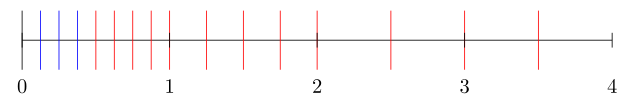
\includegraphics[width=\textwidth]{buono.png}
                \caption{e = -126}
            \end{figure}
            \begin{figure}[h]
                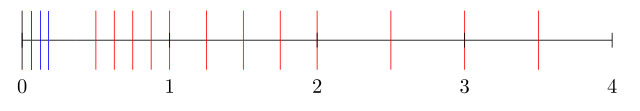
\includegraphics[width=\textwidth]{cattivo.png}
                \caption{e = -127. Da notare il gap tra blu e rosso}
            \end{figure}
        \end{center}          
        Nella rappresentazione esadecimale di un numero floating point, 
        possiamo dedurre il segno se il valore della prima cifra esadecimale
        è $>$ 0x8.
        \subsubsection{Calcolare minimo e massimo}
            Potrebbe essere utile saper calcolare il minimo 
            ed il massimo valore rappresentabile in un numero floating point, 
            ignorando ovviamente 0 e numeri negativi. \\
            Definiamo C = bit usati per la mantissa ed E = bit usati per esponente
            $$M = (2.0-2^{-C}) * 2^{2^E-2-bias}$$
            $$m = (2.0 - 1.0) * 2^{1-bias} = 2^{1-bias}$$
            $$M_D =  (1 - 2^{-C}) * 2^{1-bias}$$
            $$m_D = (2^{-C}) * 2^{1-bias}$$ 
            Per 32 bit:
            \begin{itemize}
                \item $M \approx 3.4 * 10^38$
                \item $m \approx 1.2 * 10^-38$
                \item $M_D \approx 1.2 * 10^-38$
                \item $m_D \approx 1.4 * 10^-45$
            \end{itemize}
        \subsubsection{Half precision Floating Point}
        \begin{itemize}
            \item \textbf{16 bit}: 1 segno, 5 esponente, 10 mantissa.
            \item Bias: 15.
            \item Denormalized: $(-1)^s * 2^{-14} * 0.m$.
            \item $M = 65504$
            \item $m \approx 6.1 * 10^{-5}$
            \item $M_D \approx 6.1 * 10^{-5}$
            \item $m_D \approx 5.96 * 10^{-8}$
        \end{itemize}
        \subsubsection{Double precision Floating Point}
        \begin{itemize}
            \item \textbf{64 bit}: 1 segno, 11 esponente, 53 mantissa
            \item Bias: 1023
            \item Denormalized: $(-1)^s * 2^{-1022} * 0.m$.
            \item $M \approx 1.79 * 10^{308}$
            \item $m \approx 2.2 * 10^{-308}$
            \item $M_D \approx 2.2 * 10^{-308}$
            \item $m_D \approx 2.47 * 10^{-324}$
        \end{itemize}
        \subsubsection{Approssimazioni dei Floating Points} %Vedere come completare
        \begin{itemize}                                 % questo paragrafo
            \item Problemi: \textbf{overflow} o \textbf{underflow}
            \item Soluzioni:
                \item \textbf{Toward zero}: 
                    Ignoriamo i bit dopo quelli disponibili. \\
                    1.01001, 3 bit decimali disponibili: 1.010.
                \item \textbf{To nearest}: 
                    Verso il numero più vicino. \\
                    1.100101 (1.578125), 3 bit decimali, 1.101
                \item \textbf{Down}:
                    per difetto
                \item \textbf{Up}:
                    per eccesso
        \end{itemize}
        \subsubsection{Addizione}
        \begin{enumerate}
            \item Prendere la mantisse e considerarle con la cifre sottintese
            \item Shiftare la mantissa con l'esponente minore
            \item Sommare le mantisse e normalizzare
            \item Calcolare l'esponente corretto
            \item Approssimare la mantissa
        \end{enumerate}
        \subsubsection{Moltiplicazione}
        \begin{enumerate}
            \item Sommare esponenti
            \item Prodotto mantisse
            \item Normalizzare 
        \end{enumerate}
\newpage
\section{Algebra booleana}
    \subsection{Definzioni}
        \begin{itemize}
            \item $\n{X}$: \textbf{Complemento} negato di $X$
            \item $X$ o $\n{X}$: \textbf{Literal}
            \item \textbf{Implicant}: prodotto di literal
            \item \textbf{Minterm}: prodotto di tutte le variabili d'input
            \item \textbf{Maxterm}: somma di tute le variabili d'input
            \item \textbf{Forma minima}: Forma col minor numero di min/maxtermini di un'espressione booleana
            \item \textbf{Forma canonica}: Espressione  di un circuito booleano contenente
                tutti i max/mintermini
        \end{itemize}
    \subsection{Dualità dell'algebra booleana}
        \noindent\setlength\tabcolsep{4pt}
        \def\arraystretch{2}
        \hspace*{-3.3\leftmargin}\begin{tabularx}{1.492\linewidth}{|c|c|c|}
            \hline
            Identità & $B * 1 = B$ & $B + 0 = B$ \\
            \hline
            Null element & $B * 0 = 0$ & $B + 1 = 1$ \\
            \hline
            Idempotenza & $B * B = B$ & $B + B = B$ \\
            \hline
            Involuzione & $\n{\n{B}} = B$ & $\n{\n{B}}= B$ \\
            \hline
            Complemento & $B\n{B} = 0$ & $B + \n{B} = 1$ \\
            \hline
            Commutativa & $BC = CB$ & $B + C = C + B$ \\
            \hline
            Associativa & $\left(BC\right)D = B\left(CD\right)$ & $\left(B + C\right) + D = B + \left(C + D\right)$ \\
            \hline
            Distributiva & $B\left(C + D\right) = BC + BD$ & $B + \left(CD\right) = \left(B + C\right)\left(B + D\right)$ \\
            \hline
            $1^{°}$ teorema assorbimento & $B\left(B + C\right) = B$ & $B + \left(BC\right) = B$ \\
            \hline
            $2^{°}$ teorema assorbimento & $\left(B\n{C}\right) + \left(BC\right) = B$ & $\left(B + \n{C}\right)\left(B + C\right) = B$  \\
            \hline
            Teorema della ridondanza & $\left(B\n{C}\right) + C = B + C$ & $\left(B + \n{C}\right)C = BC$ \\
            \hline
            Teorema del consenso & $\left(BC\right) + \left(\n{B}D\right) + \left(CD\right) = \left(BC\right) + \left(\n{B}D\right)$
                & $\left(B + C\right)\left(\n{B} + D\right)\left(C + D\right) = \left(B + C\right)\left(\n{B} + D\right)$ \\
            \hline
            De Morgan & $\overline{B_0 * B_1 * ...} = \overline{B_0} + \overline{B_1} + ...$ & 
                $\overline{B_0 + B_1 + ...} = \overline{B_0} * \overline{B_1} + ...$ \\
            \hline
        \end{tabularx} \\ \\ \\
        I teoremi sono dimostrabili per: \textbf{induzione perfetta}, 
        verificando la veridicita per tutti i possibili casi, oppure usando gli assiomi
        e gli altri teoremi per rendere il termine di sinistra uguale a quello di destra 
    \subsection{Mappe di Karnaugh}
        Le k-maps sono uno strumento grafico di minimazzione di espressioni booleane, 
        usate quando si hanno fino a 5 varabili (dopo diventa particolarmente scomodo). \\
        Consiste nel creare una tabella, fino a 4 variabili, o 2 tabelle, per 5 variabili,
        contenti i possibili stati delle variabili della nostra espressione.
        \begin{center}
                \begin{figure}[H]
                    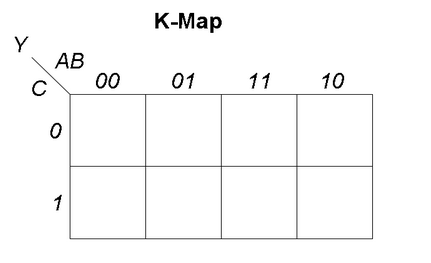
\includegraphics[width=.3\textwidth]{k1.png}\hfill
                    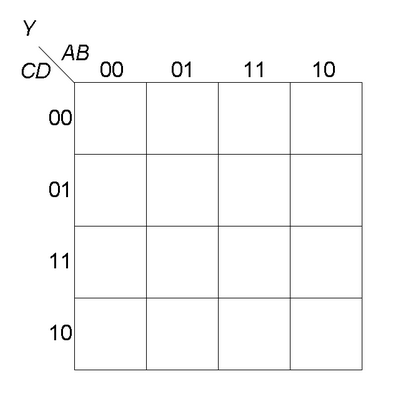
\includegraphics[width=.3\textwidth]{k2.png}\hfill
                    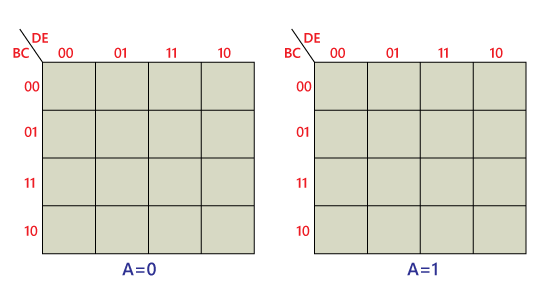
\includegraphics[width=.3\textwidth, height = 2.5cm]{k3.png}
                \end{figure}
        \end{center}
        \subsubsection{Regole delle k-maps}
        \begin{itemize}
            \item Ogni casella corrisponde ad un mintermine
            \item Ogni 1 deve essere cerchiato almeno una volta
            \item Ogni cerchio deve selezionare $2^\alpha$ 1
            \item Ogni cerchio deve essere il più grande possibile
            \item Un cerchio può andare da angoli opposti ad angoli opposti
            \item I \textbf{don't care} vengono presi solo se aiutano a minimizzare l'equazione
            \item Il cerchio più grande è detto \textbf{Prime Implicant}
        \end{itemize}
            Queste sono le regole per ottenere una SOP, per la POS basta prendere gli 0 ed i maxtermini.
    \subsection{Teorema di shannon}
        $f(x_1, x_2, ..., x_n) = x_1 * f(1, x_2, ..., x_n) + \n{x_1} * f(0, x_2, ..., x_n)$
        Dal teorema possiamo dedurre che qualsiasi circuito combinatorio ad n variabili 
        è realizzabile con un multiplexer e due circuiti ad n-1 variabili.            
\newpage
\section{Circuiti logici}
    \subsection{Porte logiche}
        Componente che svolge una funzione logica elementare. \\
        Può avere da 1 a n input ed 1 output. 
        \subsubsection{NOT}
        Nega il valore in entrata
        \begin{center}
            \begin{figure}[H]
                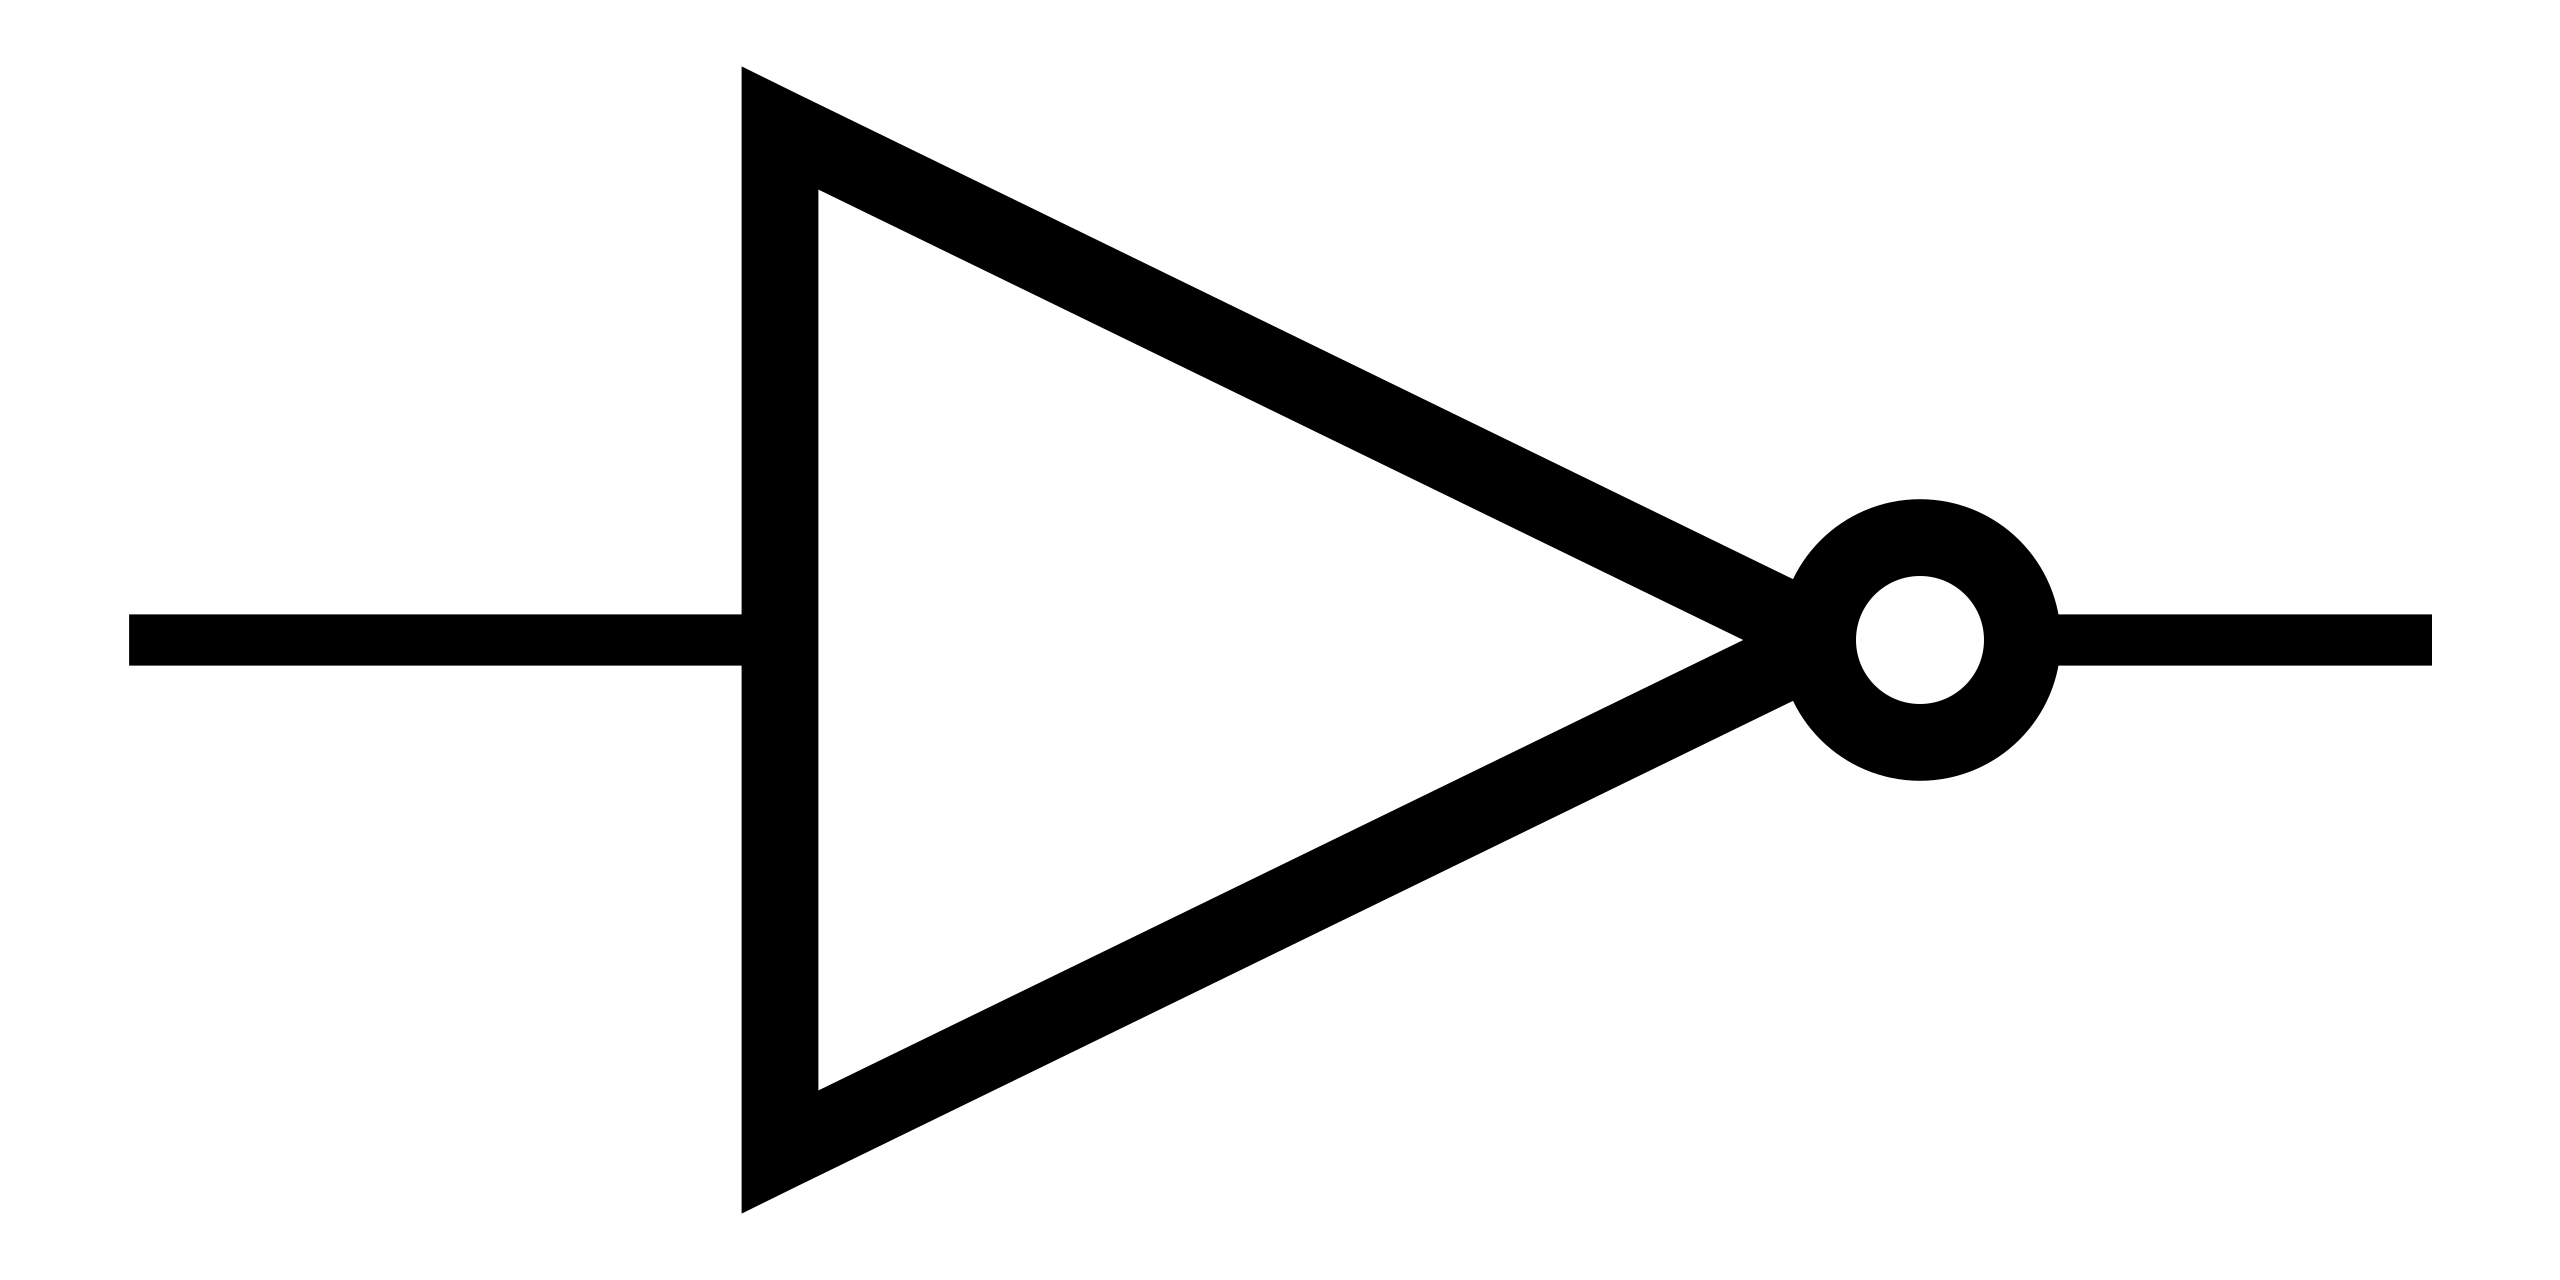
\includegraphics[width=2cm,height=1cm]{not.png}
            \end{figure}
        \end{center}
        \subsubsection{BUFFER}
            Usato per pulire il segnale
            \begin{center}
                \begin{figure}[H]
                    
\includegraphics[width=2cm,height=1cm]{buffer.png}
                \end{figure}
            \end{center}
        \subsubsection{AND}
            Prodotto logico
            \begin{center}
                \begin{figure}[H]
                    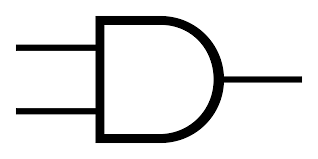
\includegraphics[width=2cm,height=1cm]{and.png}
                \end{figure}
            \end{center}
        \subsubsection{OR}
            Somma logica
            \begin{center}
                \begin{figure}[H]
                    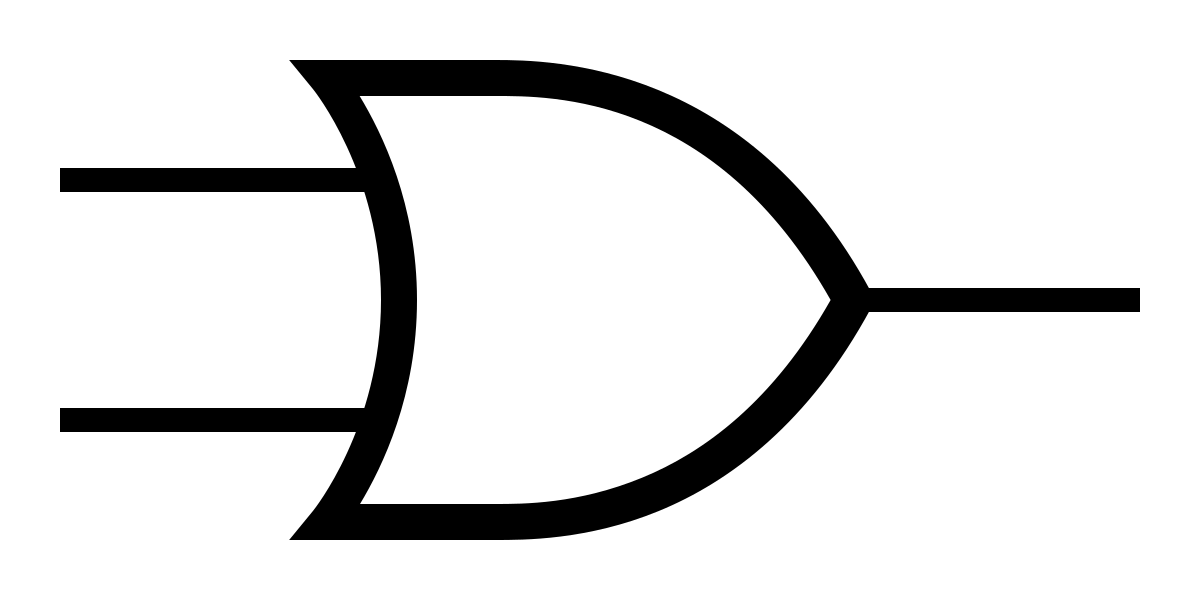
\includegraphics[width=2cm,height=1cm]{or.png}
                \end{figure}
            \end{center}
        \subsubsection{XOR}
            Somma logica esclusiva
            \begin{center}
                \begin{figure}[H]
                    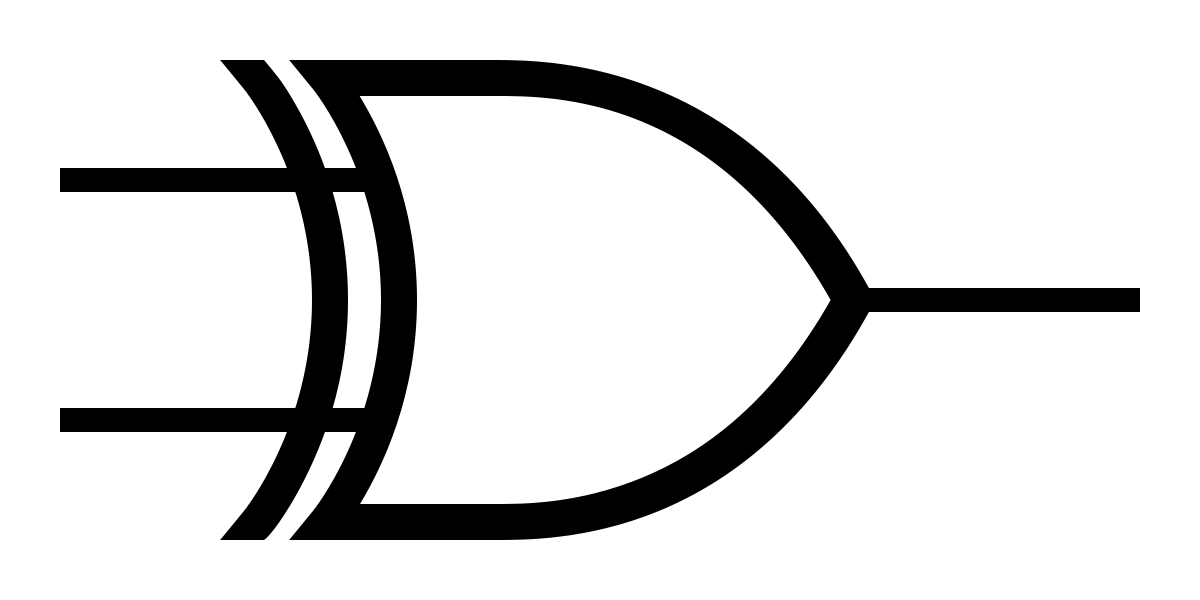
\includegraphics[width=2cm,height=1cm]{xor.png}
                \end{figure}
            \end{center}
        \subsubsection{NAND}
            AND seguito da NOT
            \begin{center}
                \begin{figure}[H]
                    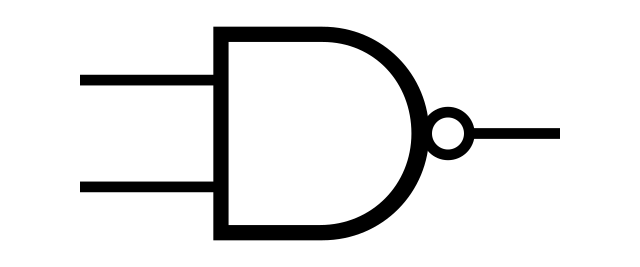
\includegraphics[width=2cm,height=1cm]{nand.png}
                \end{figure}
            \end{center}
        \subsubsection{NOR}
            OR seguito da NOT
            \begin{center}
                \begin{figure}[H]
                    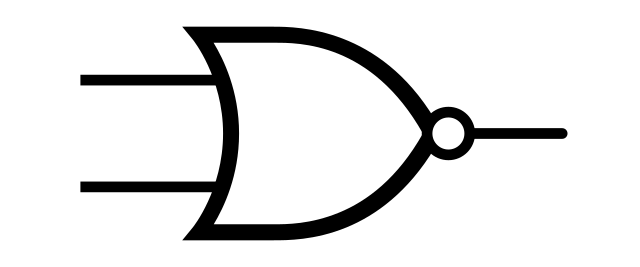
\includegraphics[width=2cm,height=1cm]{nor.png}
                \end{figure}
            \end{center}
        \subsubsection{XNOR (Anche noto come EQ)}
            XOR seguito da NOT
            \begin{center}
                \begin{figure}[H]
                    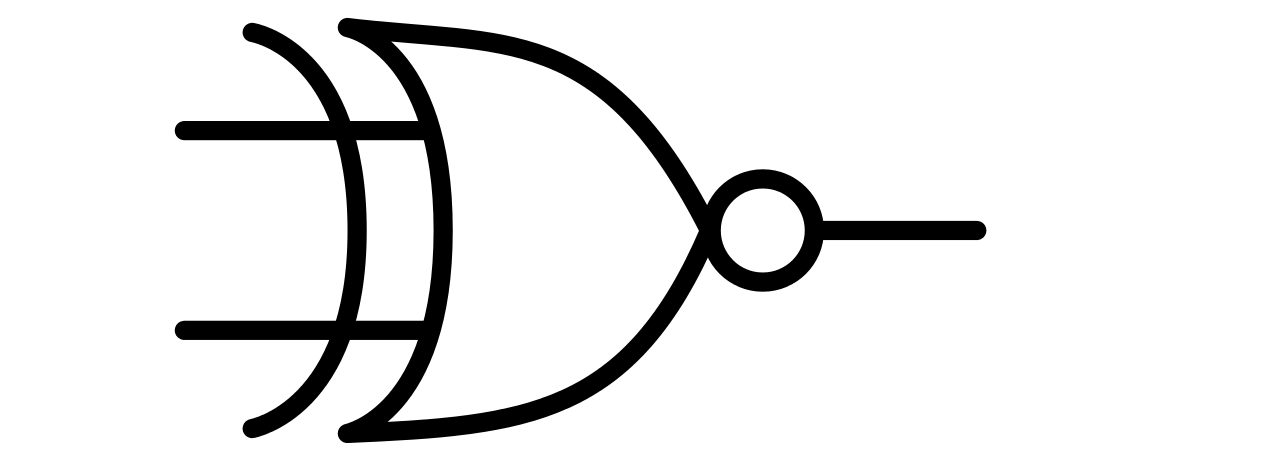
\includegraphics[width=2cm,height=1cm]{xnor.png}
                \end{figure}
            \end{center}
    \subsection{Descrivere circuito come operazioni logiche}
        \subsubsection{Sum-of-products form}
        \begin{enumerate}
            \item Scrivere tabella verità
            \item Scrivere i \textbf{minterm} m che, presi gli input A e B delle
              proprie corrispondenti righe, restituisce \textbf{1}
            \item Scegliere i minterm delle righe con $y=1$ e nominarli progressivamente $k_i$
            \item $y = \Sigma_{i=0}^{\#K}k_i$
        \end{enumerate}
        \subsubsection{Product-of-sums form}
        \begin{enumerate}
            \item Scrivere tabella verità
            \item Scrivere i \textbf{maxterm} M che, presi gli input A e B delle
            proprie corrispondenti righe, restituisce \textbf{0}
            \item Scegliere i maxterm delle righe con $y=0$ e nominarli progressivamente $k_i$
            \item $y = \Pi_{i=0}{\#K}k_i$
        \end{enumerate}
    \subsection{Bubble pushing}
        De Morgan ci permette di vedere, a livello circuitale, la correttezza 
        del \textbf{bubble pushing}, ovvero l'uguaglianza fra una porta logica e 
        la sua porta "opposta" con input ed output negati rispetto l'originale.
        \begin{center}
            \begin{figure}[H]
                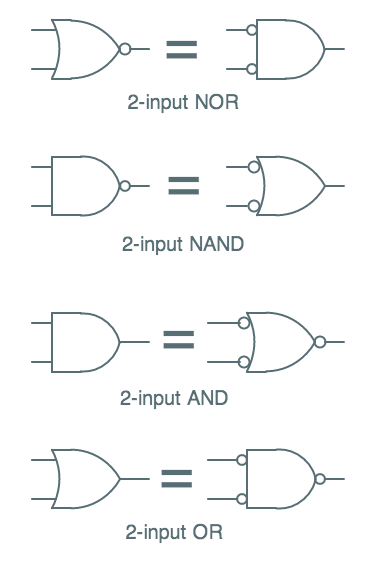
\includegraphics[width=\textwidth]{bubblepushing.png}
            \end{figure}
        \end{center}  
    \subsection{NAND e NOR}
        \subsubsection{Universalità}
            \begin{center}
                \begin{figure}[H]
                    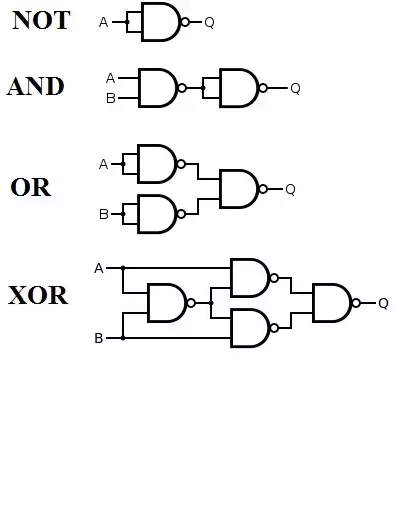
\includegraphics[width=\textwidth]{completeness.png}
                \end{figure}
            \end{center}  
        \subsubsection{Convenienza}
            Conviene usare NAND e NOR piuttosto che OR ed AND in quanto sono
            realizzabili con meno transistor
        \subsection{Non associatività}
            Suddette porte logiche non godono della proprietà associativa     
    \subsection{Multiple output circuits}
        I circuiti possono avere anche molteplici output. \\
        In questo caso risulta facili pensare ad ogni output come ad un circuito a 2
        livelli a parte, ma nella realtà non è fatto così in quanto nella maggior parte 
        dei casi porterebbe all'uso di un numero maggiore di porte logiche e a circuiti
        più costosi e più lenti.
    \subsection{Codifica one-hot}
        La codifica one-hot è un tipo di codifica usata nei ciruiti a N input e/o 
        N output dove solo uno dei bit ha il valore \textbf{1}
    \subsection{Don't cares}
        Segnalati nelle tabelle di verità e nelle k-maps con una \textbf{"X"}, indicano
        valori per i quali non ci interessa sapere se sono 1 o 0.
    \subsection{Contention}
        Una contention accade quando il circuito tenta di avere sia 0 che 1 come output. \\
        Questa condizione indica spesso un bug nel circuito e viene indicato col simbolo \textbf{"X"}.
    \subsection{Floating}
        Un nodo flottante può avere come output 0, 1 od un valore nel mezzo, indicato col 
        simbolo \textbf{"Z"}. \\
        In questa condizione si può considerare il nodo come un \textbf{interruttore aperto}. \\
        Questa proprietà è sfruttata per realizzare i \textbf{tristate buffers}.
        \begin{center}
            \begin{figure}[H]
                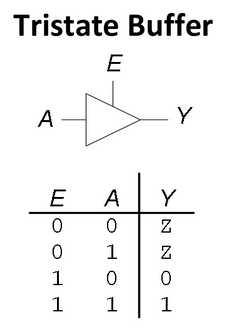
\includegraphics[width=\textwidth]{tristatebuffer.png}
            \end{figure}
        \end{center}  
    \subsection{Tristate busses}
        I tristate buffer sono usati per la costruzione dei \textbf{tristate busses},
        con la promessa che solo un buffer alla volta sia attivo
        \begin{center}
            \begin{figure}[H]
                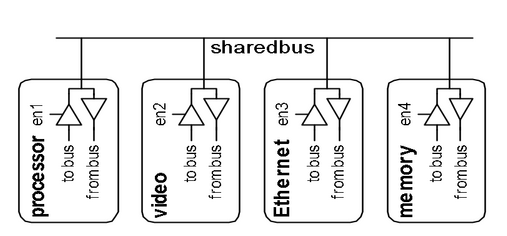
\includegraphics[width=\textwidth]{tristatebusses.png}
            \end{figure}
        \end{center}      
    \subsection{Circuiti ad n-livelli}
        Volendo, potremmo comporre tutti i circuiti combinatori a 2 livelli, 
        ma nella realtà difficilmente si fa questa scelta, poichè capita di 
        frequente che all'interno di un circuito ci siano porte logiche riutilizzabili
        più volte, costruendo quindi un circuito più piccolo e con meno porte logiche, 
        il che ci porta dei vantaggi di \textbf{area} occupata e \textbf{calore} generato dal circuito,
        al netto delle \textbf{performance}.
    \subsection{Multiplexer}
        Il MUX è un circuito con N input, $\log_2N$ input di selezione e 
        1 output, e vengono realizzati coi \textbf{tristate busses}. \\
        Con i multiplexer 2:1 e \textbf{possibile realizzare qualsiasi circuito combinatorio} 
        (\textbf{lookup table}), e vengono usati in quanto usano pochi transistor.
    \subsection{Decoder}
        Il DEC è un circuito con 1 input dati, N output di uscita e $\log_2N$
        input di selezione, che scelgono su quale output mandare il segnale. \\
        Il DEC realizza tutti i possibili mintermini di un espressione con $\log_2N$
        variabili, ed usandoli è quindi \textbf{possibile realizzare qualsiasi circuito combinatorio}.
    \subsection{Delay}
        Il delay è il tempo che ci impiega un circuito a modificare l'output quando
        si modificano gli input, ed è causato dalle proprietà intrinsiche delle porte logiche (capacità e resistenze) e 
        dal limite della velocità della luce. \\
        Questo tempo è \textbf{diverso} in base a quali input cambiano, a come cambia l'output e 
        allo stato del circuito (freddo / caldo), e quindi non esiste un delay universale per la porta logica. \\
        Si individuano quindi 2 delay:
        \begin{itemize}
            \item \textbf{propagation delay}: t$_{pd}$, il delay \textbf{massimo}
            \item \textbf{contamination delay}: t$_{cd}$, il delay \textbf{minimo}
        \end{itemize}
        \subsubsection{Critical e short path}
            La critical path sarebbe il tempo \textbf{massimo} che il circuito ci mette, cambiato 
            un input, a cambiare l'output, La short path quello \textbf{minimo}.
            Il tempo della CP si calcola sommando i t$_{pd}$ delle porte che compongono la CP,
            quello della SP sommando i t$_{cd}$ delle porte che compongono la SP
            \begin{center}
                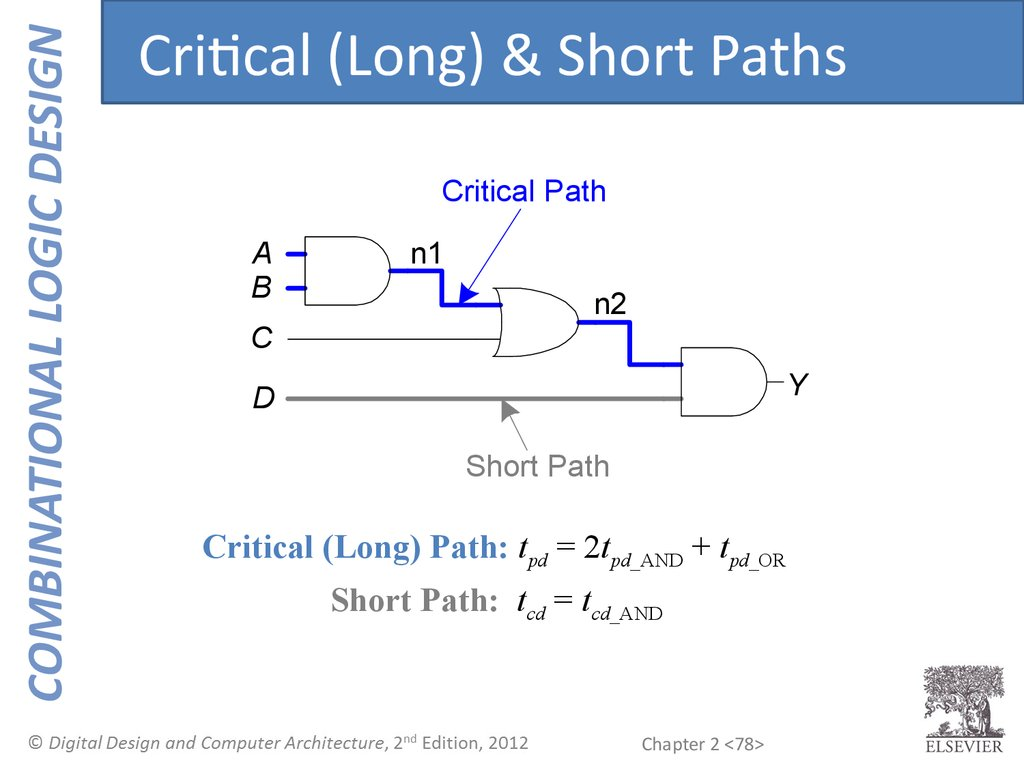
\includegraphics[width=\textwidth]{path.jpg}
            \end{center}
\newpage
\section{Circuiti logici combinatori}
    \begin{itemize}
        \item \textbf{Memoryless}
        \item No percorsi \textbf{ciclici}
        \item Ogni nodo è un input o si collega a un \textbf{solo} output
        \item Out = $f$(Input)
        \item Composti da sottocircuiti combinatori
    \end{itemize}
\section{Circuiti logici sequenziali}
    \begin{itemize}
        \item \textbf{Memoria short-term}, ovvero finchè il circuito rimane alimentato
        \item Presentano uno \textbf{Stato}
        \item Out = $f$(Input, State)
    \end{itemize}
    \subsection{Componenti dei circuiti bistabili}
        \subsubsection{Circuiti bistabili}
            Sono il blocco elementare dei circuiti sequenziali. \\
            Presentano 2 stati, $Q$ e $\n{Q}$, ma nessun input. \\
        \subsubsection{Latch S-R}
            \begin{center}
                \begin{figure}[h]
                    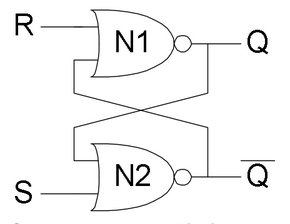
\includegraphics[width=0.5\textwidth, height=4cm]{latchsr.png}
                    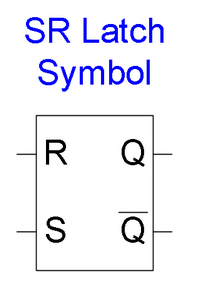
\includegraphics[width=.5\textwidth, height=4cm]{latchsr2.png}
                \end{figure}
            \end{center}
            \begin{itemize}
                \item S = 1, R = 0 $\Longrightarrow$ Q = 1
                \item S = 0, R = 1 $\Longrightarrow$ Q = 0
                \item S = 0, R = 0 $\Longrightarrow$ Q = Q$_{prev}$
                \item S = 1, R = 1 $\Longrightarrow$ Q = Invalid (da evitare)
            \end{itemize}
        \subsubsection{Latch D}
            \begin{center}
                \begin{figure}[H]
                    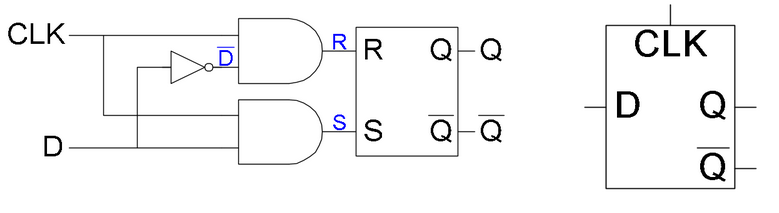
\includegraphics[width=\textwidth, height=4cm]{latchd.png}
                \end{figure}
            \end{center}
            Input:
            \begin{itemize}
                \item \textbf{Clock} (CLK): definisce quando l'output deve cambiare (0 hold, 1 trasparente rispetto a D)
                \item D: Il valore da memorizzare
            \end{itemize}
            Funzionamento:
            \begin{itemize}
                \item CLK = 0, D = X $\Longrightarrow$ Q = Q$_{prev}$
                \item CLK = 1 $\Longrightarrow$ Q = D
            \end{itemize}
        \subsubsection{Problematiche dei latch}
            I latch presentano la problematica che, all'interno dello stesso periodo
            di clock, \textbf{l'output può variare più volte in tempi brevissimi, aumentando lo 
            spreco d'energià e la complessità nella progettazione del circuito}. \\
            La soluzione sono i flip-flop, dispositivi \textbf{edge-triggered}, nei quali lo stato di trasparenza occorre 
            in corrispondenza del \textbf{fronte di salita}(o discesa) del CLK. \\
            Nel nostro caso li consideriamo tutti sul fronte di salita
        \subsubsection{Flip-Flop D}
            \begin{center}
                \begin{figure}[H]
                    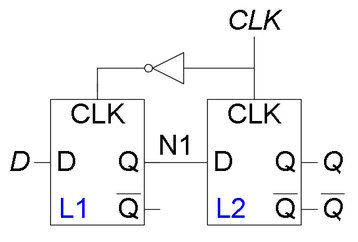
\includegraphics[width=0.5\textwidth, height=4cm]{flipflopd.png}
                    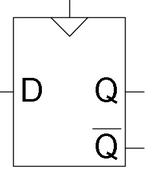
\includegraphics[width=0.5\textwidth, height=4cm]{flipflopd2.png}
                \end{figure}
            \end{center}
            \begin{itemize}
                \item CLK = 0, CLK$_{prev}$ = X, D = X $\Longrightarrow$ Q = Q$_{prev}$
                \item CLK = 1, CLK$_{prev}$ = 1, D = X $\Longrightarrow$ Q = Q$_{prev}$
                \item CLK = 1, CLK$_{prev}$ = 0 $\Longrightarrow$ Q = D
            \end{itemize}
        \subsubsection{Enabled F-F}
            \begin{center}
                \begin{figure}[H]
                    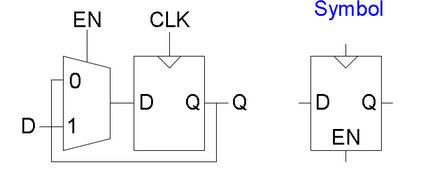
\includegraphics[width=0.67\textwidth, height=4cm]{flipflope.png}
                    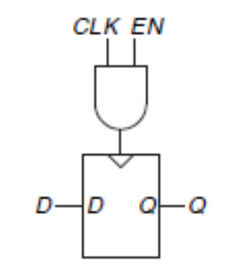
\includegraphics[width=0.33\textwidth, height=4cm]{flipflope2.png}
                \end{figure}
            \end{center}
            \begin{itemize}
                \item EN = 0 $\Longrightarrow$ Funziona come F-F D
                \item EN = 1 $\Longrightarrow$ Q = Q$_{prev}$
            \end{itemize}
        \subsubsection{Resettable e Settable F-F}
            Queste 2 tipologie di F-F sono usate per circuiti nei quali è importante 
            partire da uno stato noto dopo l'accensione del sistema (es: centrali elettriche). \\
            Possono essere:
            \begin{itemize}
                \item Sincroni: l'output cambia quando il segnale di set/reset = 1 e CLK è sul fronte di salita/discesa
                \item Asincroni: l'output cambia quando il segnale di set/reset = 1, senza considerare CLK. 
                    Richiedono un cambiamento del circuito interno del F-F.
            \end{itemize}
            \subsubsubsection{Resettable F-F}
                \begin{center}
                    \begin{figure}[H]
                        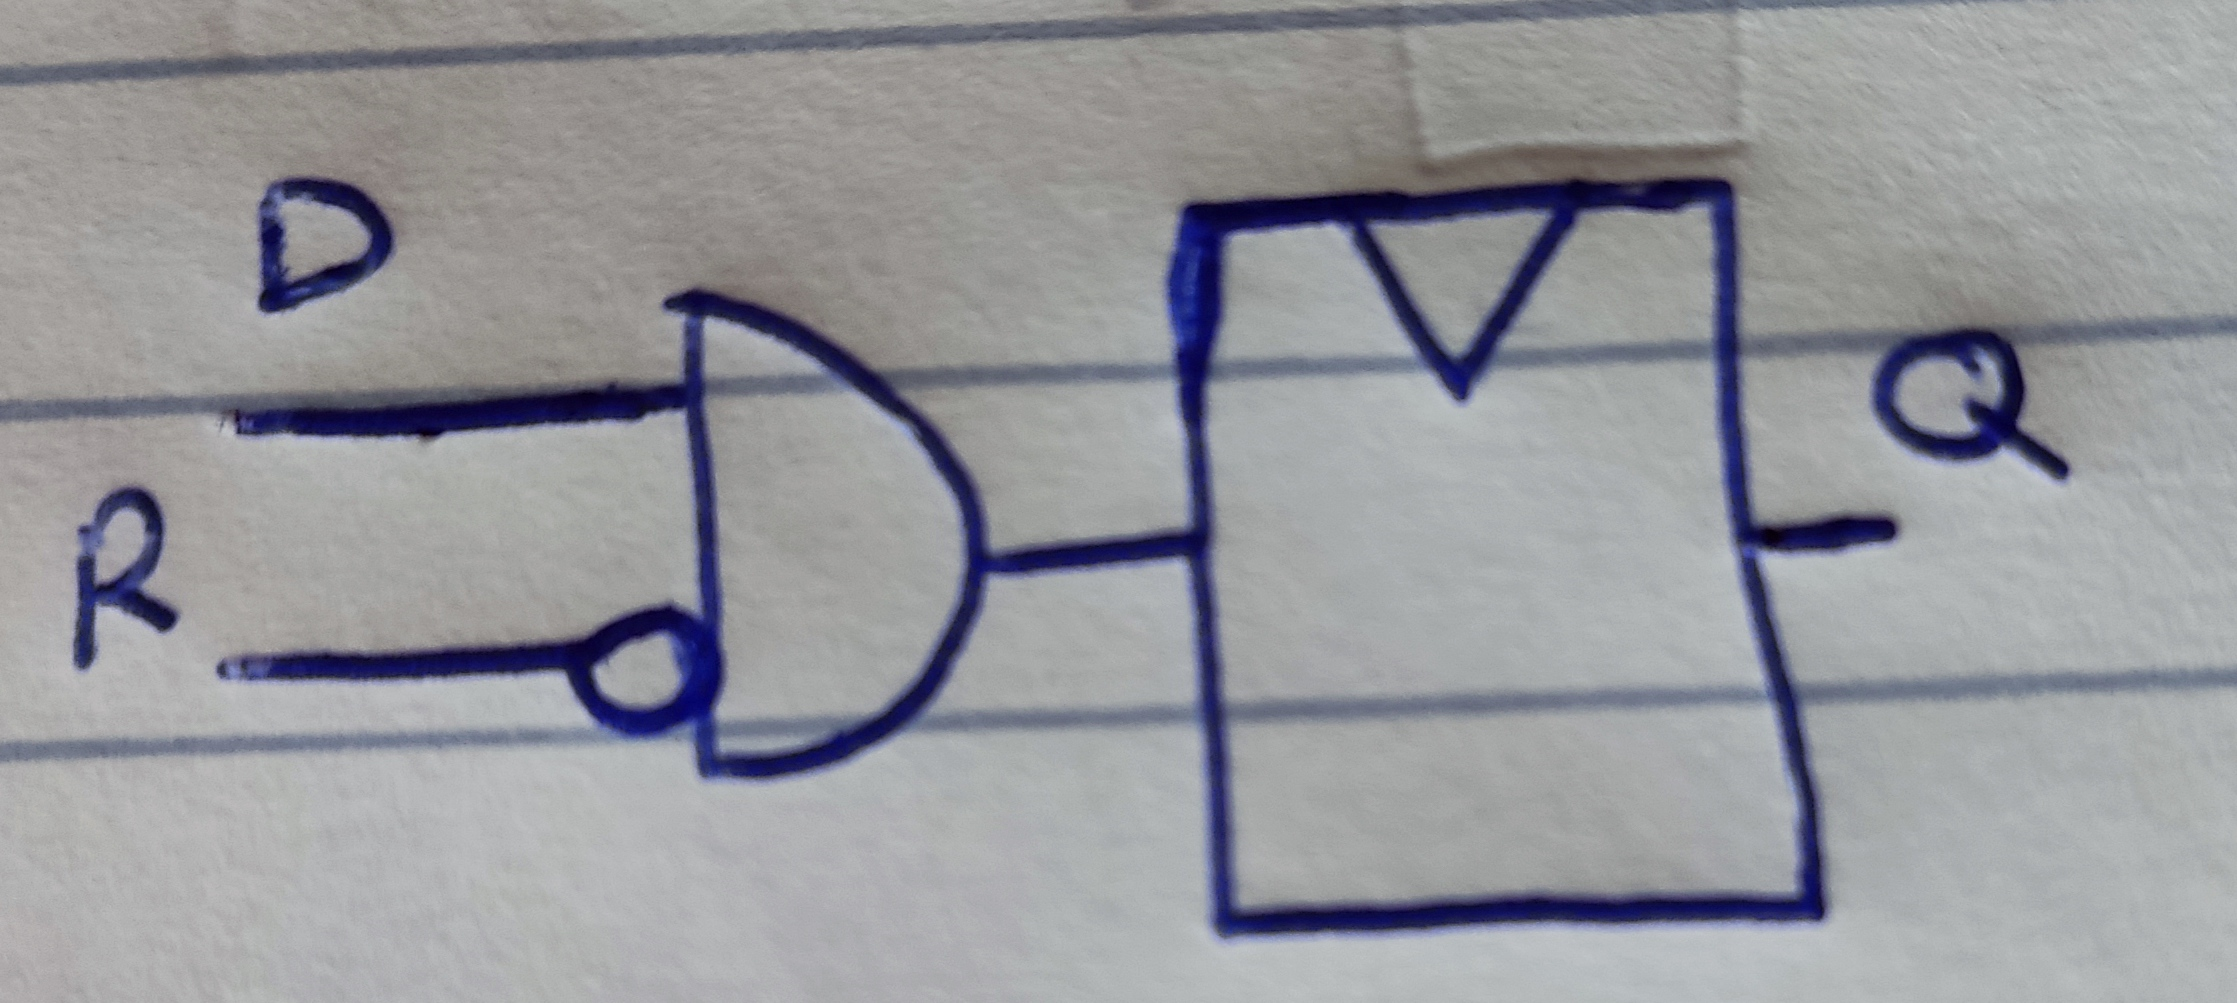
\includegraphics[width=0.5\textwidth, height=4cm]{flipflopr.jpg}
                        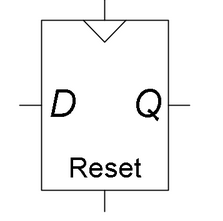
\includegraphics[width=0.5\textwidth, height=4cm]{flipflopr2.png}
                    \end{figure}
                \end{center}
                \begin{itemize}
                    \item R = 0 $\Longrightarrow$ Funziona come F-F D
                    \item R = 1 $\Longrightarrow$ Q = 0
                \end{itemize}
            \subsubsubsection{Settable F-F}
                \begin{center}
                    \begin{figure}[H]
                        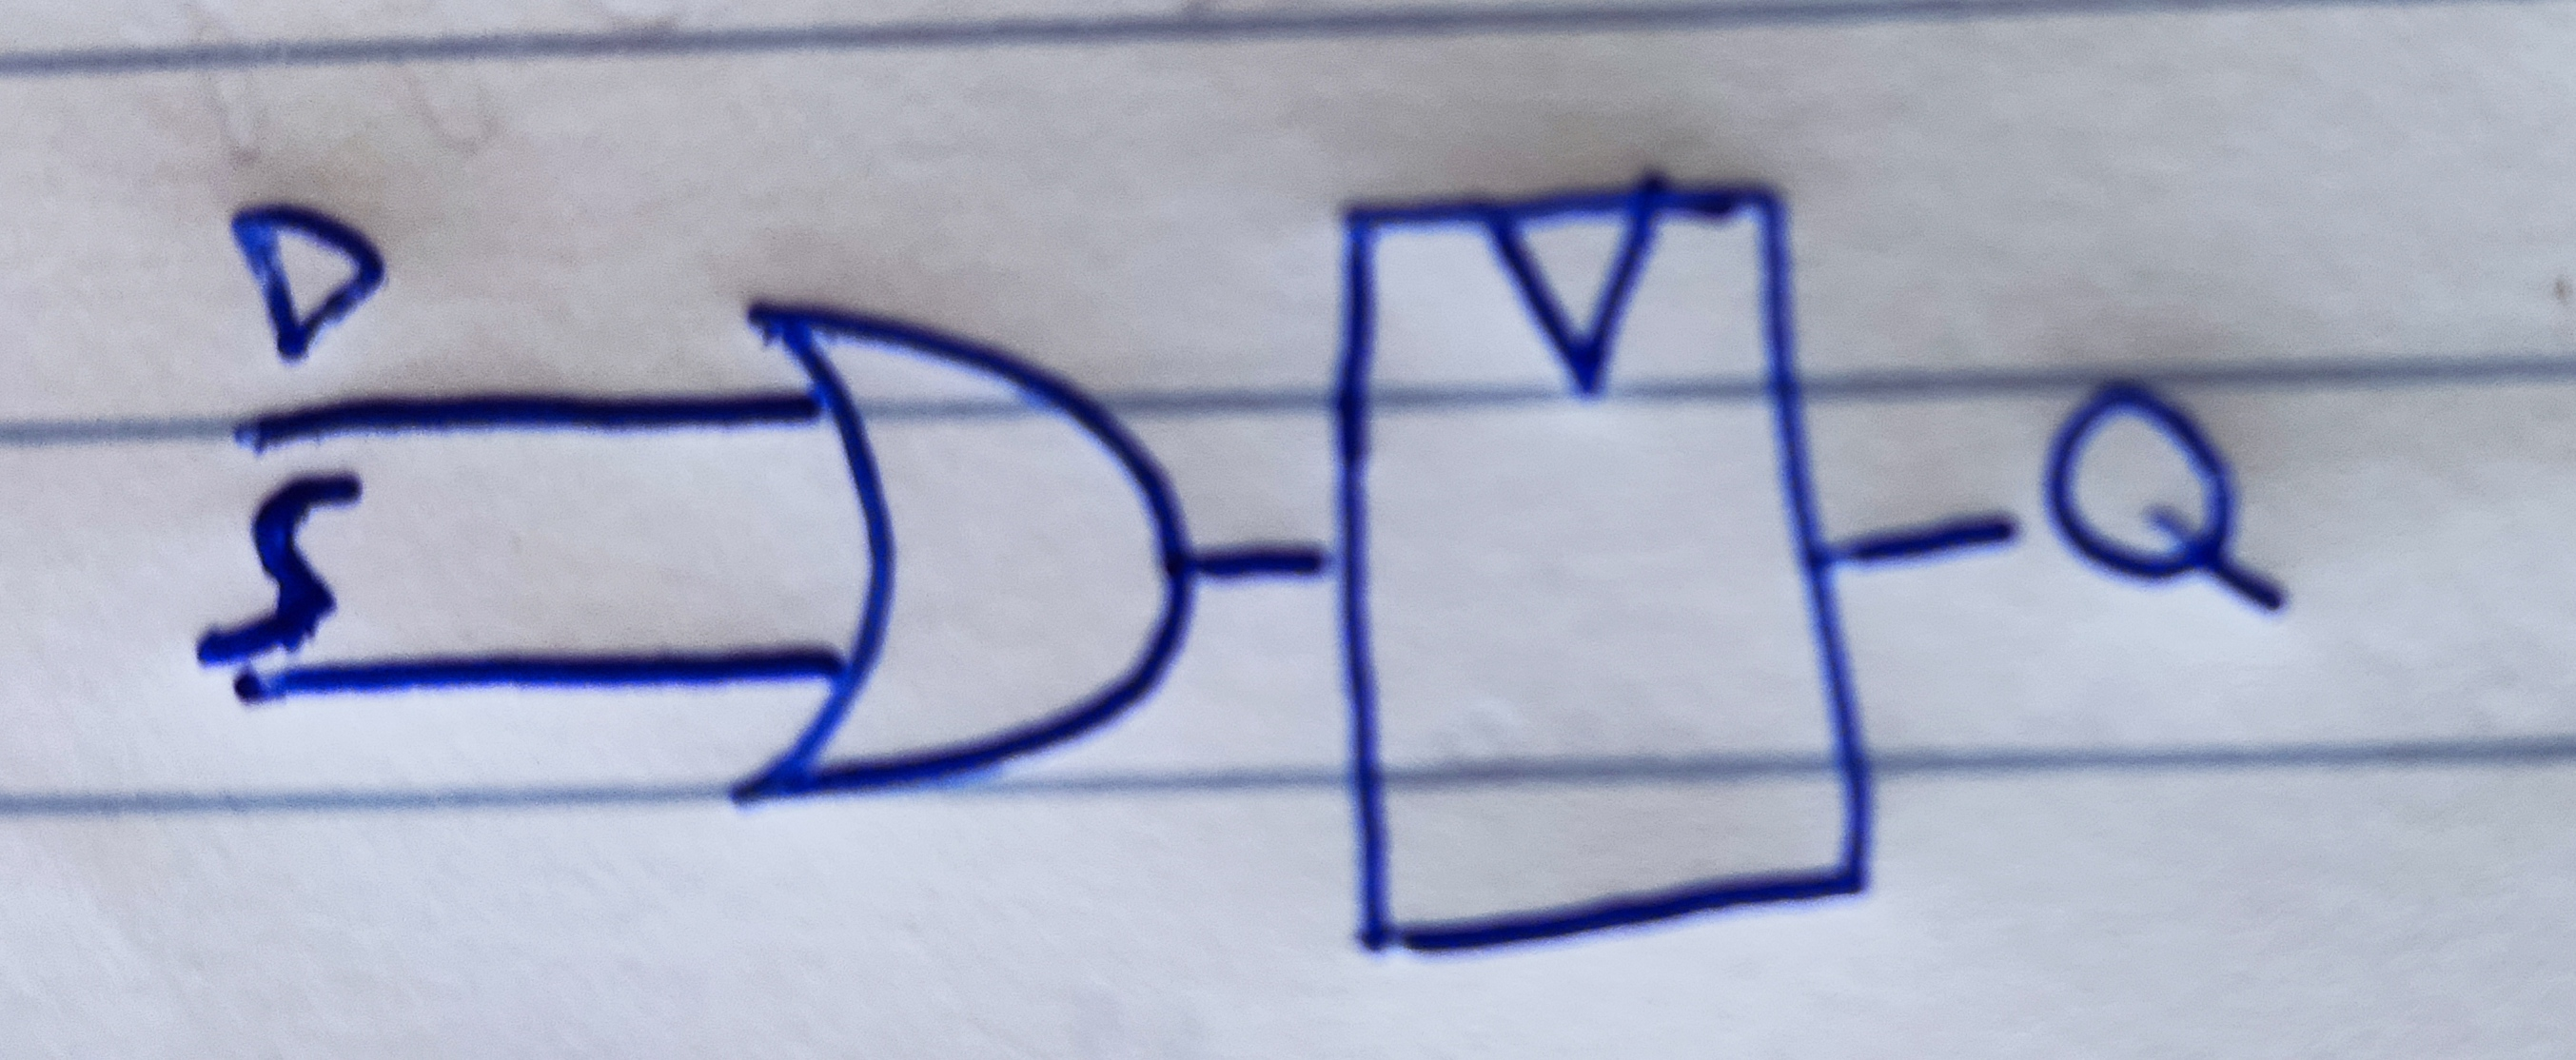
\includegraphics[width=0.5\textwidth, height=4cm]{flipflops.jpg}
                        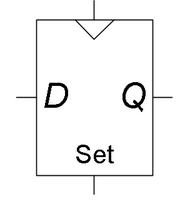
\includegraphics[width=0.5\textwidth, height=4cm]{flipflops2.png}
                    \end{figure}
                \end{center}
                \begin{itemize}
                    \item S = 0 $\Longrightarrow$ Funziona come F-F D
                    \item S = 1 $\Longrightarrow$ Q = 1
                \end{itemize}
        \subsubsection{Registri}
            I \textbf{registri} sono \textbf{batterie di F-F}
            \begin{center}
                \begin{figure}[H]
                    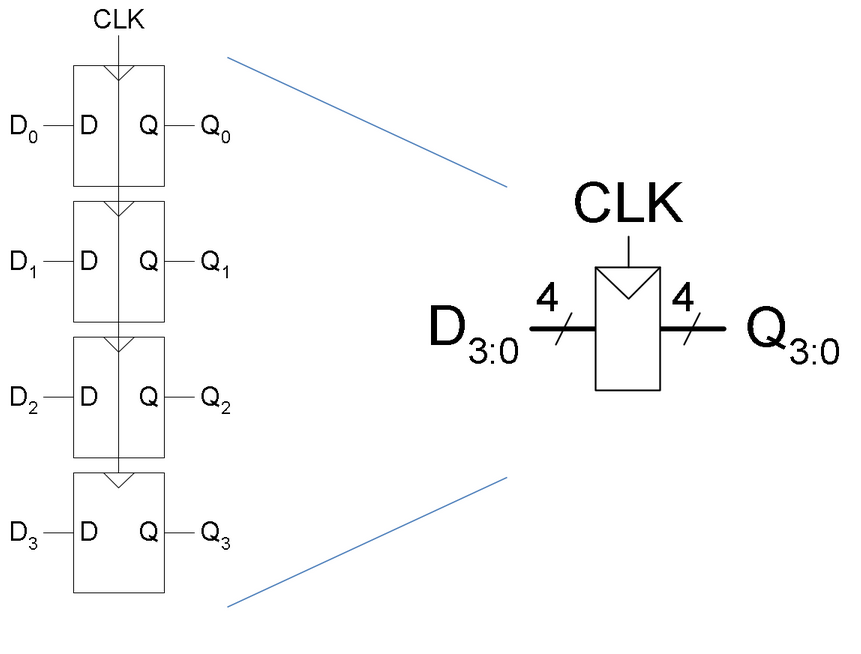
\includegraphics[width=\textwidth]{registri.png}
                \end{figure}
            \end{center}
    \subsection{Regole della progettazione dei circuiti logici sequenziali sincroni}
        \begin{itemize}
            \item \textbf{Spezzare} tutte le path cicliche con almeno 1 registro, 
                che memorizza \textbf{lo stato del sistema}, per path
            \item Sincronizzare sul CLK: lo stato viene aggiornato sul \textbf{fronte di salita}(o discesa) del CLK
            \item Tutti i registri sono \textbf{sincronizzati sullo stesso CLK}
            \item E' composto da almeno \textbf{1 registro} e \textbf{circuiti combinatori}
        \end{itemize}
    \subsection{Macchine a stati finiti}
        Le macchine a stati finiti (\textbf{FSM}), sono circuiti composti da 1
        \textbf{registro di stato} e \textbf{due circuiti combinatori}, 1 che 
        \textbf{calcola il prossimo stato} sulla base degli input e dello stato corrente,
        e uno che \textbf{calcola gli output}. \\
        Si dividono in FSM di Moore e FSM di Mealy.
        \subsubsection{FSM di Moore}
            $$S^{'} = f_{S}\left(I, S\right)$$
            $$Out = f_{Out}\left(S\right)$$
            \begin{center}
                \begin{figure}[H]
                    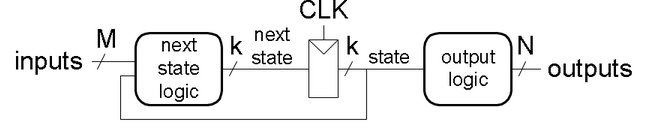
\includegraphics[width=\textwidth, height=3cm]{moorefsm.png}
                \end{figure}
            \end{center}
        \subsubsection{FSM di Mealy}
            $$S^{'} = f_{S}\left(I, S\right)$$
            $$Out = f_{Out}\left(I, S\right)$$
            \begin{center}
                \begin{figure}[H]
                    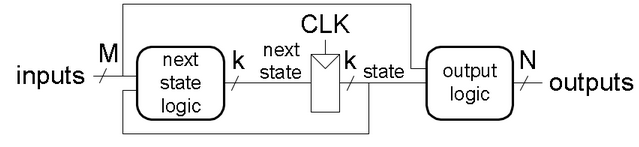
\includegraphics[width=\textwidth, height=3cm]{mealyfsm.png}
                \end{figure}
            \end{center}
        \subsubsection{Progettazione di una FSM}
            \begin{enumerate}
                \item Definiamo gli In e gli Out
                \item Disegnamo il diagramma di transizione:
                    \begin{itemize}
                        \item Nodi: rappresentano lo stato, all'interno contengono 
                            i valori dell'output in quello stato
                        \item Archi: Transizione. Possono presentare gli input 
                            che inducono in quello stato (non sempre presenti)
                    \end{itemize}
                \item Costruiamo la tabella di transizione
                \item Costruiamo la tabella di transizione codificata
                \item Definiamo l'equazioni degli stati codificati
                \item Costruiamo l'output table codificata
                \item Definiamo l'equazioni degli output codificati
                \item Costruiamo il circuito
                \item Costruiamo il diagramma del tempo
                \end{enumerate}
        \subsubsection{Esempio dei semafori}
            \subsubsubsection{Problema}
                Abbiamo un incrocio gestito da 2 coppie di semafori, che
                regolano il traffico sulla strada orizzontale A e su quella verticale B,
                e che presenta 2 sensori di traffico, per vedere se sono presenti macchine
                sulle strade. \\
                E' permesso il passaggio su una sola strada alla volta.
                Procediamo a progettare la FSM.
            \subsubsubsection{Input e Output}
                Gli input sono i due sensori, T$_A$ e T$_B$, che assumono il valore
                di 0 quando la strada è libera e 1 quando è occupata, gli output sono
                L$_A$ e L$_B$, che assumono i valori R, Y, G (sono quindi due coppie di valori 
                binari per output).
            \subsubsection{Diagramma di transizione}
                \begin{itemize}
                    \item 0) Stato di partenza (reset state): L$_A$ = G, L$_B$ = R. Lo stato è mantenuto finchè c'è traffico sulla strada A
                    \item 1) Quando non c'è più traffico sulla strada A, passiamo allo stato dove L$_A$ = Y, L$_B$ = R.
                    \item 2) Al prossimo CLK passiamo allo stato con L$_A$ = R, L$_B$ = G, mantenuto finchè c'è traffico sulla strada B
                    \item 3) Quando non c'è più traffico sulla strada B, passiamo allo stato dove L$_A$ = R, L$_B$ = Y
                    \item 0) Al prossimo CLK torniamo allo stato 0
                \end{itemize}
                Il diagramma ottenuto è:
                \begin{center}
                    \begin{figure}[H]
                        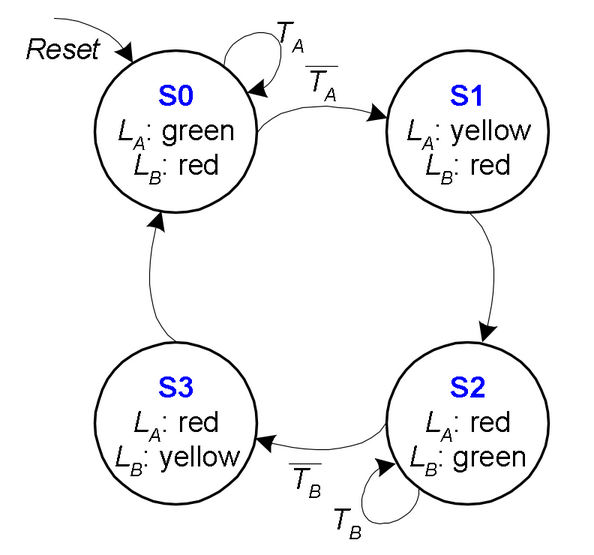
\includegraphics[width=\textwidth, height=5cm]{fsmd.png}
                    \end{figure}
                \end{center}
            \subsubsubsection{Tabella di transizione}
                \begin{center}
                    \begin{tabular}{|c|c|c|c|}
                        \hline
                        Current State & T$_A$ & T$_B$ & Next State \\
                        \hline
                        S$_0$ & 0 & X & S$_1$ \\
                        \hline
                        S$_0$ & 1 & X & S$_0$ \\
                        \hline
                        S$_1$ & X & X & S$_2$ \\
                        \hline
                        S$_2$ & X & 0 & S$_3$ \\
                        \hline
                        S$_2$ & X & 1 & S$_2$ \\
                        \hline
                        S$_3$ & X & X & S$_0$ \\
                        \hline
                    \end{tabular}
                \end{center}
            \subsubsubsection{Tabella di transizione codifica}
                Tabella di codifica degli stati:
                \begin{center}
                    \begin{tabular}{|c|c|c|}
                        \hline
                        State & Encoding \\
                        \hline
                        S$_0$ & 00 \\
                        \hline
                        S$_1$ & 01 \\
                        \hline
                        S$_2$ & 10 \\
                        \hline
                        S$_3$ & 11 \\
                        \hline
                    \end{tabular}
                \end{center}
                Tabella di transizione codificata:
                \begin{center}
                    \begin{tabular}{|c|c|c|c|c|c|}
                        \hline
                        ES$_0$ & ES$_1$ & T$_A$ & T$_B$ & ES$^{'}_0$ & ES$^{'}_1$ \\
                        \hline
                        0 & 0 & 0 & X & 0 & 1 \\
                        \hline
                        0 & 0 & 1 & X & 0 & 0 \\
                        \hline
                        0 & 1 & X & X & 1 & 0 \\
                        \hline
                        1 & 0 & X & 0 & 1 & 1 \\
                        \hline
                        1 & 0 & X & 1 & 1 & 0 \\
                        \hline
                        1 & 1 & X & X & 0 & 0 \\
                        \hline
                    \end{tabular}
                \end{center}
            \subsubsection{Equazioni stati codificato}
                $$ES^{'}_0 = ES_0 \oplus ES_1$$
                $$ES^{'}_1 = \n{ES_0} * \n{ES_1} * \n{T_A} + \n{ES_0}ES_1\n{T_B}$$
            \subsubsubsection{Tabella di output codificata}
                Tabella di codifica degli output
                \begin{center}
                    \begin{tabular}{|c|c|}
                        \hline
                        Out & Encoding \\
                        \hline
                        G & 00 \\
                        \hline
                        Y & 01 \\
                        \hline
                        R & 10 \\
                        \hline
                    \end{tabular}
                \end{center}
                Tabella di output codificata:
                \begin{center}
                \begin{tabular}{|c|c|c|c|c|c|}
                    \hline
                    ES$_0$ & ES$_1$ & L$_{A0}$ & L$_{A1}$ & L$_{B0}$ & L$_{B1}$ \\
                    \hline
                    0 & 0 & 0 & 0 & 1 & 0 \\
                    \hline
                    0 & 1 & 0 & 1 & 1 & 0 \\
                    \hline
                    1 & 0 & 1 & 0 & 0 & 0 \\
                    \hline
                    1 & 1 & 1 & 0 & 0 & 1 \\
                    \hline
                \end{tabular}
                \end{center}
            \subsubsubsection{Equazioni output codificati}
                $$L_{A0} = ES_0$$
                $$L_{A1} = \n{ES_0}ES_1$$
                $$L_{B0} = \n{ES_0}$$
                $$L_{B1} = ES_0ES_1$$
            \subsubsubsection{Circuito}
                \begin{center}
                    \begin{figure}[H]
                        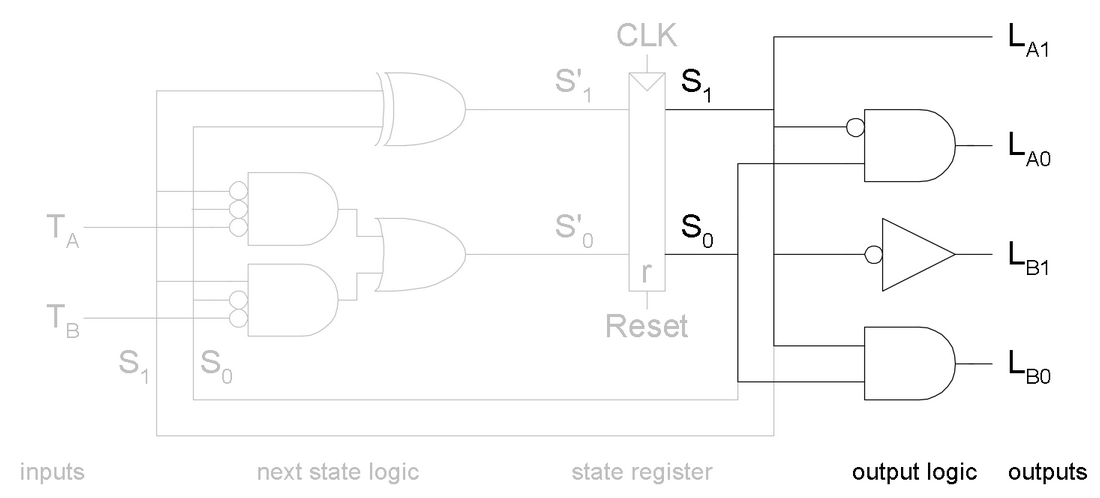
\includegraphics[width = \textwidth, height = 5cm]{fsmc.png}
                    \end{figure}
                \end{center}
            \subsubsubsection{Tabella del tempo}
                \begin{center}
                    \begin{figure}[H]
                        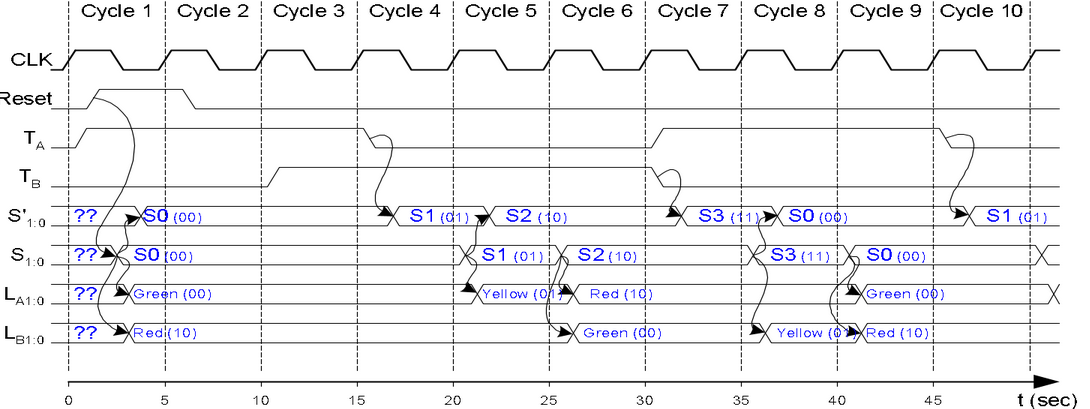
\includegraphics[width = \textwidth, height = 5cm]{fsmt.png}
                    \end{figure}
                \end{center}

            



                



    

     

         
        


\end{document}

